\documentclass[10pt,final]{beamer}
\mode<presentation>
\usetheme{lucasdeb}
\usepackage{debiantutorial}

\hypersetup{pdftitle={Practical session 2: gnujump},bookmarks}
\title[Practical session 2: gnujump]{Practical session 2:\\ Packaging GNUjump}
\author[]{Lucas Nussbaum\\{\small\texttt{lucas@debian.org}}}
\institute{
\includegraphics[viewport=274 335 360 440,width=1cm]{figs/openlogo-nd.pdf}}
\date{}

\begin{document}

\frame{\titlepage}

\begin{frame}{Practical session: packaging GNUjump}
\begin{enumerate}
	\item Download GNUjump 1.0.6 from
		\url{http://ftp.gnu.org/gnu/gnujump/1.0.6/gnujump-1.0.6.tar.gz}
		\br
	\item Create a Debian package for it
		\begin{itemize}
			\item Install build-dependencies so that you can build the package
			\item Get a basic working package
			\item Finish filling \texttt{debian/control} and other files
		\end{itemize}
		\br
	\item Enjoy
\end{enumerate}
\vfill
\centerline{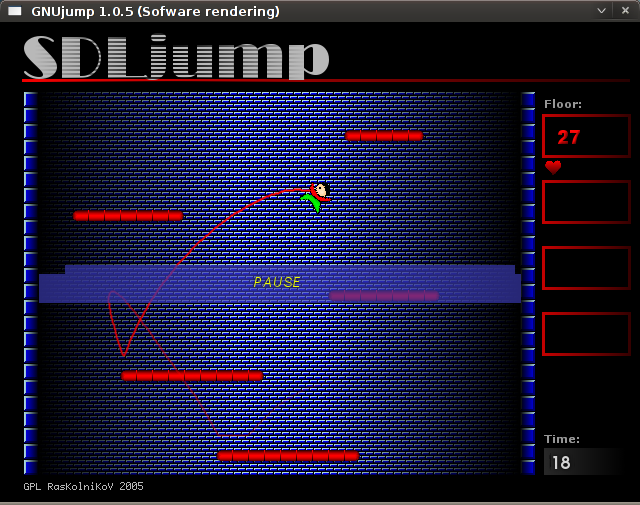
\includegraphics[width=6cm]{gnujump.png}}
\end{frame}

\begin{frame}[fragile]
\frametitle{Step by step\ldots}
\begin{itemize}
	\item \texttt{wget http://ftp.gnu.org/gnu/gnujump/1.0.6/gnujump-1.0.6.tar.gz}
		\hbr
	\item \texttt{mv gnujump-1.0.6.tar.gz gnujump\_1.0.6.orig.tar.gz}
		\hbr
	\item \texttt{tar xf gnujump\_1.0.6.orig.tar.gz}
		\hbr
	\item \texttt{cd gnujump-1.0.6/}
		\hbr
	\item \texttt{dh\_make}
	\begin{itemize}
		\item \small Type of package: single binary (for now)
	\end{itemize}
\end{itemize}
\begin{lstlisting}[basicstyle=\ttfamily\small]
gnujump-1.0.6$ ls debian/
changelog           gnujump.default.ex   preinst.ex
compat              gnujump.doc-base.EX  prerm.ex
control             init.d.ex            README.Debian
copyright           manpage.1.ex         README.source
docs                manpage.sgml.ex      rules
emacsen-install.ex  manpage.xml.ex       source
emacsen-remove.ex   menu.ex              watch.ex
emacsen-startup.ex  postinst.ex
gnujump.cron.d.ex   postrm.ex
\end{lstlisting}
\end{frame}

\begin{frame}[fragile]
\frametitle{Step by step \ldots (2)}
\begin{itemize}
	\item Look at \texttt{debian/changelog}, \texttt{debian/rules}, \texttt{debian/control} (auto-filled by \textbf{dh\_make})
	\item In \texttt{debian/control}:\\
		\texttt{Build-Depends: debhelper (>= 7.0.50~), autotools-dev}
		This field lists the \textsl{build-dependencies}: packages needed to build the package
	\item Try to build the package as-is (thanks to \textbf{dh} magic)
		\begin{itemize}
			\item And add build-dependencies, until it builds
			\item Hint: use \texttt{apt-cache search} and \texttt{apt-file} to find the packages
			\item Example:
\begin{lstlisting}[basicstyle=\ttfamily\footnotesize]
checking for sdl-config... no
checking for SDL - version >= 1.2.0... no
[...]
configure: error: *** SDL version 1.2.0 not found!
\end{lstlisting}
$\rightarrow$ Add \textbf{libsdl1.2-dev} to Build-Depends and install it.
		\end{itemize}
\end{itemize}
\end{frame}

\begin{frame}
\frametitle{Step by step \ldots (3)}
\begin{itemize}
	\item After installing \texttt{libsdl1.2-dev, libsdl-image1.2-dev, libsdl-mixer1.2-dev}, the package builds fine.
		\hbr
	\item Use \texttt{debc} to list the content of the generated package.
		\hbr
	\item Use \texttt{debi} to install it and test it.
		\hbr
	\item Fill in \texttt{debian/control} using \url{http://www.debian.org/doc/debian-policy/ch-controlfields.html}
		\hbr
	\item Test the package with \texttt{lintian}
		\hbr
	\item Remove the files that you don't need in \texttt{debian/}
		\hbr
	\item Compare your package with the one already packaged in Debian:
		\begin{itemize}
			\item It splits the data files to a second package, that is the same across all architectures ($\rightarrow$ saves space in the Debian archive)
			\item It installs a .desktop file (for the GNOME/KDE menus) and also integrates into the Debian menu
			\item It fixes a few minor problems using patches
		\end{itemize}
\end{itemize}
\end{frame}
\end{document}
